\documentclass[10pt]{article}
\usepackage[]{graphicx}
\usepackage{caption}
\usepackage{subfigure}
\usepackage{amsmath}
\usepackage{float}
%\usepackage{epsfig}
\usepackage{lipsum}
\usepackage[margin=1in]{geometry}
\usepackage{multicol}
\usepackage{abstract}
\usepackage{indentfirst}
\renewcommand{\abstractnamefont}{\normalfont\bfseries} % Set the "Abstract" text to bold
\renewcommand{\abstracttextfont}{\normalfont\small\itshape} % Set the abstract itself to small italic text

\setlength{\columnsep}{0.3in}

\author{Apoorva Bansal, Jay Patel, Vivek Gokuladas}
\title{Discovering Panoramas in Web Videos}
\date{\today}

\begin{document}
\maketitle


% Abstract:
\begin{abstract}
In this project, we present a method to discover panoramic source frames within web videos. The project is based on existing paper \cite{Feng}.  Videos are a good source for panoramas as camera panning naturally creates a wide field-of-view of a scene. But the problem is challenging because many of the videos are recorded casually, without the intent of capturing a panorama. Our method finds segments within a video that are good candidates for panorama sources. Finding these segments requires extracting the different scenes in the video. After finding these segments, we keep the ones that achieve an optimal balance between maximizing the visual quality and the wide field-of-view. Once these segments are discovered, good quality panoramas are synthesized using them.  Our method was able to detect good quality panoramas in videos with high accuracy. We ran experiments on various web videos to confirm its feasibility and to demonstrate the utility of this method. 
\end{abstract}




% Report:
\begin{multicols}{2}
% 1 Introduction:
\section{Introduction}
A panoramic image is a wide angle view of a particular scene. Panoramic imagery can be found in many places 
and has been used throughout history as a method to showcase large scenes in their entirety. Often, it is 
difficult to take photographs of a wide field-of-view without specialized equipement. As a result, research
in computer vision has identified methods in panorama stitching that combine multiple images with some 
overlap into a single panoramic image. Videos provide a source in which the likelihood of a panorama is high;
when a video pans, each frame overlaps with the previous to form a series of images with a wide field-of-view.
\par
Panorama stitching algorithms consist of two main steps; aligning images together by calculating homography
values between image pairs followed by blending them together to provide a clean transition between images.
Most algorithms also require that the input images have been identified as high quality and are supplied in 
the correct order ready for alignment and blending. Additionally, panoramas are restricted by the supply of
photographs of the physical destination. 
\par 
In these times, there exist vast caches of pictures and videos made available online through services such as
YouTube \cite{YouTube}, Vimeo \cite{Vimeo}, Picasa \cite{Picasa}, and many more. These resources can provide access
to multimedia content pertaining to many places around the world. Video sources have especially become common
for many of the popular places around the world, with many of these having the potential for becoming future
panoramas. Some of these videos are not of high quality and thus cannot be used to create a panorama. In an 
effort to identify these videos, we use three conditions; a video must cover a wide field-of-view, the video
must satisfy the thresholds for each image quality critereon, and that the video provides frames that relate
to each other through homographies and are not an individual collection of separate images.
\par
In this paper, we apply the strategy of panorama discovery in web videos identified in Liu et al \cite{Feng} 
with some improvements to shot detection and panorama discovery. A large part of our implementation focuses
on detecting panoramas compared with the majority of research being done on panorama stitching. This focus
is important as it allows users to automate the process of readying media for panorama stitching and provides
a framework for discovering panoramas automatically from videos. We have split our design into five specific 
parts, shot detection, homography calculation, quality calculation, panorama discovery, and image stitching. 
The overall flow and how these parts are connected is shown in Figure (\ref{fig:HLD}).
\end{multicols}

\begin{figure}[t] 
  \centering
  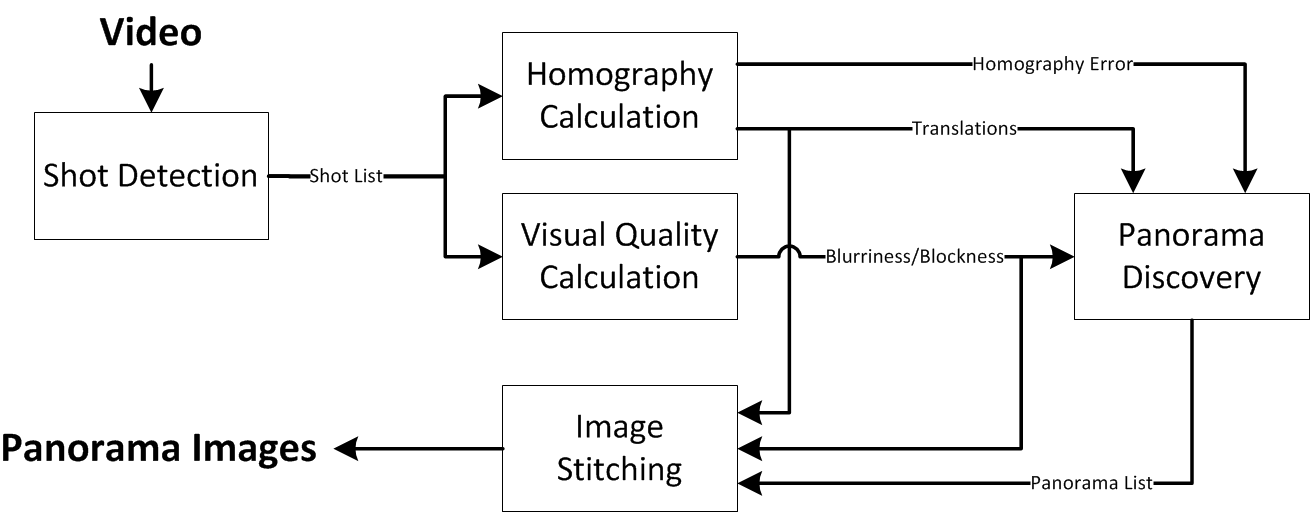
\includegraphics[scale=1.2]{HLD.png}  
  \caption{High Level Diagram.} \label{fig:HLD}
\end{figure}

\begin{multicols}{2}
% 2 Contributions:
\section{Contributions}

% 2.1 Previous Work:
\subsection{Previous Work}


% 2.2 Improvements:
\subsection{Improvements}


% 3 Technical Solution:
\section{Technical Solution}
Our technical solution summary is discussion in Section (\ref{sec:TechSolSummary}) and details are discussed in Section (\ref{sec:TechSolDetails}).

% 3.1 Summary:
% 3.1 Summary:
\subsection{Summary} \label{sec:TechSolSummary}

The technical solution used to extract panoramas from web videos is split into different steps shown in Figure (\ref{fig:HLD}).  
A video clip is first divided into a sequence of shots using a shot boundary detection algorithm.  
A shot is defined as a continuous frame sequence recorded by a camera setting.  We implemented an edge detection based method to identify shots.  
The next step is homography and visual quality calculation.  Homographies between frames were determined using SIFT and RANSAC.  
We assumed no skew or rotation in the homographies to simplify our stitching implementation.  
Visual quality of each frame was determined using a Blurriness and Blockness algorithm.  
Our implementation of the Blurriness algorithm was based on a paper by Tong et al \cite{Tong}.  
Our implementation of the Blockness algorithm was based on a paper by Wang et al \cite{Wang}.  The next step is panorama discovery.  
This is viewed as a computationally difficult optimization problem.  
The optimization problem is meant to find a balance between maximizing visual quality and scene extent.  
We implemented an approximation of this optimization problem.  The last step is image stitching.  We implemented a three stage blending algorithm.  
The stages were feathering, median bilateral filter, and visual quality weighting.  The end result is the discovered panoramas from the video clip.



% 3.2 Details:
% 3.2 Details:
\subsection{Details} \label{sec:TechSolDetails}
Each major component of our technical solution shown in Figure (\ref{fig:HLD}) is discussed in the following subsections. 

\subsection{Shot Detection} \label{sec:ShotDetect}
The video can be split into a sequence of shots. Each shot is defined as a continuous frame sequence of shots. Each shot is defined as a continuous frame sequence recorded by a camera setting. 
Different shots most likely contain different scenes. So we break a video into a shot sequence and discover panoramas from each shot independently. We evaluated couple of methods to find the shots in the video. 
The first method we implemented was based on color histogram-based shot boundary detection \cite{Lien}. Its basic idea is that color content does not change rapidly within but across shots.
Thus, hard cuts can be detected as single peaks in the time series of the differences between color histograms of contiguous frames. 


Let $p_{i}(r,g,b)$ be the number of pixels of color (r,g,b) in frame $I_{i}$ of N pixels. Each color component is discretized to $2^{B}$ different values, resulting in r,g,b $\epsilon$ $[0, 2^{B-1}]$. Usually B is set to 2 or 3 in order to reduce sensitivity to noise and slight light, object as well as view changes. 
Then, the color histogram difference between two color frames $I_{i-1}$ and $I_{i}$ is given by

\begin{equation}
	CHD_{i} = \frac{1}{N}.\sum _{r=0}^{2^B-1}\sum _{g=0}^{2^B-1}\sum _{b=0}^{2^B-1} \mid p_{i}(r,g,b) - p_{i-1}(r,g,b) \mid
\end{equation}
	
A hard cut or a scene transition is detected when $CHD_{i}$ exceeds a certain threshold. This method didn�t perform well on all our data sets. This is because; the color histogram approach ignores the spatial distribution information of various colors.  
If the shot boundary has similar RGB color composition to its previous frame, it fails to detect the scene boundary. So we implemented a second method for shot boundary detection using edge detection. 
Here it finds the edges using a canny edge detector on frame $I_{i-1}$ and $I_{i}$. Next, it divided these edge detected frames into blocks. Now the difference of the mean of every block of the edge image $I_i$ with the mean of every block of previous image $I_{i-1}$ is taken. 
When this difference exceeds a threshold, a scene boundary is detected. A scene boundary detection depends on two threshold parameters, one is the difference threshold and the other threshold is the number of blocks where the difference of the means exceeds the difference threshold. 
After various trial and error experiments, these thresholds have been adjusted to find the hard and soft transitions. In the following sub sections, we describe the video analysis components necessary for discovering and stitching panoramas.


\begin{figure} [H]
	\centering
	\subfigure[]{
		\centering
		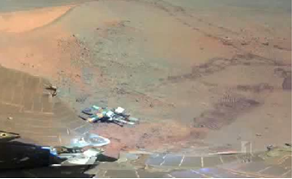
\includegraphics[width=35mm,height=35mm]{shota.png}  
		\label{fig:shota}	
	}
	\subfigure[]{
		\centering
		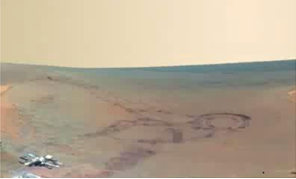
\includegraphics[width=35mm,height=35mm]{shotb.png}  
		\label{fig:shotb}
	}	
	\subfigure[]{
		\centering
		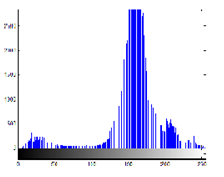
\includegraphics[width=35mm,height=35mm]{shotc.png}  
		\label{fig:shotc}	
	}
	\subfigure[]{
		\centering
		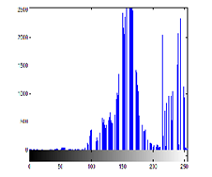
\includegraphics[width=35mm,height=35mm]{shotd.png}  
		\label{fig:shotd}
	}
	\caption{Example of a scene transition which is a soft cut that is undetected by color histogram method. a) and b) are two contiguous frames and b) is a scene transition boundary. c) and d) are the red channel histograms of a) and b) respectively. } \label{fig:shot}	
\end{figure}





\subsection{Homography Calculation} \label{sec:HomoSec}

The homography is determined between consecutive frames in order to align images.  
SIFT is used to extract feature points of every frame.  
We integrated the SIFT demo program provided by David Lowe \cite{Lowe} in our technical solution to expedite the process.  
The RANSAC algorithm is used to obtain a robust homography from matching points between two sequential frames.  
$H$ shown in equation (\ref{eq:HMat}) is the constrained homography model we used in our RANSAC implementation.  
We assumed no skew or rotation in the homographies to simplify our image stitching implementation.  
As a result, there were only translations between frames.  The translations are used in discovering panoramas and image stitching.

\begin{equation} \label{eq:HMat}
H=
\left[ \begin{array}{ccc}
1 & 0 & t_{x} \\
0 & 1 & t_{y} \\
0 & 0 & 1 \end{array} \right]
\end{equation}

The homography error is used as a measure for the motion model accuracy.  
It is calculated as the average of second norm errors of each point.   
The error of each point is between the matching SIFT feature point and calculated point from the homography.  





\subsection{Visual Quality Calculation} \label{sec:BlurBlockSec}

Visual quality calculation is used to measure the distortion of the source image.  
Many web videos are of low quality for a variety of reasons.  
They are typically highly compressed for web-sharing, causing blurring and blocking artifacts.  
Image distortion is measured as a combination of blurriness extend and blockiness extent.

\subsubsection{Blurriness}

Our implementation of the Blurriness algorithm was based on a paper by Tong et al \cite{Tong}.  
The blurriness algorithm is based on the edge type and sharpness analysis using Harr wavelet transform.  
Generally edges are classified into three types; Dirac Structure, Step-Structure, and Roof-Structure.  
In the paper by Tong et al \cite{Tong}, Step-Structure is further classified into Astep-Structure and Gstep-Structure.   
The algorithm measures the extent of blurriness as a ratio.  The ratio is the number of likely blurred 
Gstep-Structure and Roof-Structure edges to the total number of Gstep-Structure and Roof-Structure edges.  
The classification of edges is obtained from a set of rules applied to the edge maps.  
The steps to acquire the edge maps are shown below.  
The blurriness extent is demonstrated in Figure (\ref{fig:cityOriginal}) and Figure (\ref{fig:cityBlurry}).

\vspace{5 mm}

\noindent\textbf{Step 1}: Perform Harr wavelet transform to the original image and the decomposition level is 3.  
The result is a hierarchical pyramid-like structure shown in Figure (\ref{fig:PyraStruc}).

\vspace{5 mm}

\noindent\textbf{Step 2}: Construct the edge map in each scale (i=1,2,3).
\begin{equation}
Emap_{i}(k,l)=\sqrt{LH_{i}^{2}+HL_{i}^{2}+HH_{i}^{2}}  
\end{equation}

\vspace{5 mm}

\noindent\textbf{Step 3}: Partition the edge map and find the local maxima in each window.  
The window size in the highest scale is 2 x 2, the next coarser scale is 4 x 4, and the coarsest one is 8 x 8.  
The result will be the final edge map.

\vspace{5 mm}

\begin{figure}[H] 
  \centering
  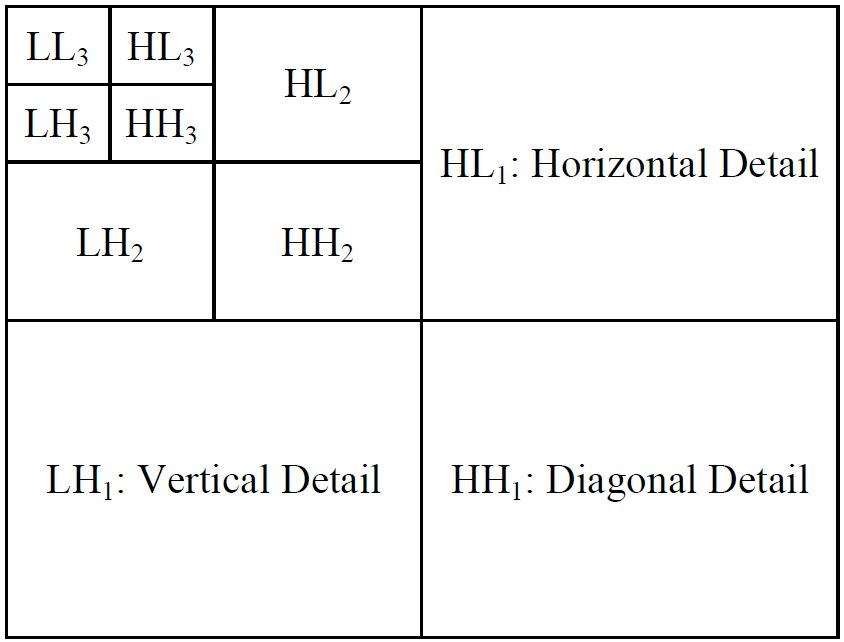
\includegraphics[scale=0.3]{pyramidStructure.jpg}  
  \caption{Pyramid of images with related sub-bands. \cite{Tong}} \label{fig:PyraStruc}
\end{figure}

\begin{figure} [H]
	\centering
	\subfigure[Blurriness = 0.2058]{
		\centering
		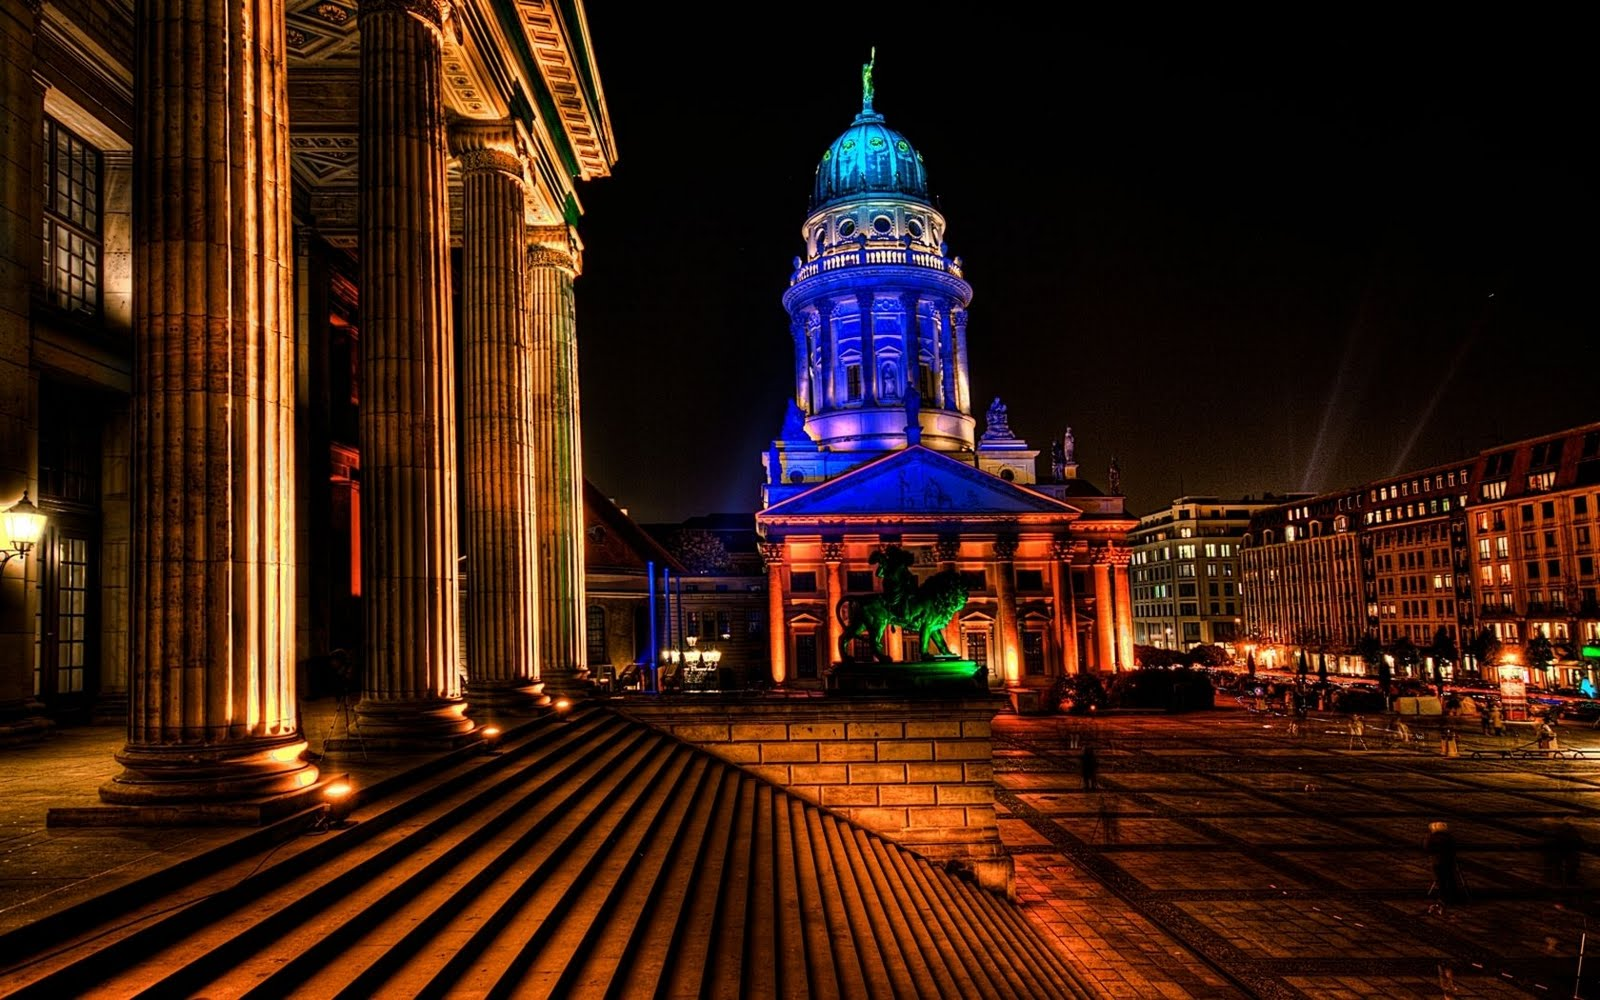
\includegraphics[width=35mm,height=35mm]{cityOriginal.jpg}  
		\label{fig:cityOriginal}	
	}
	\subfigure[Blurriness = 0.7557]{
		\centering
		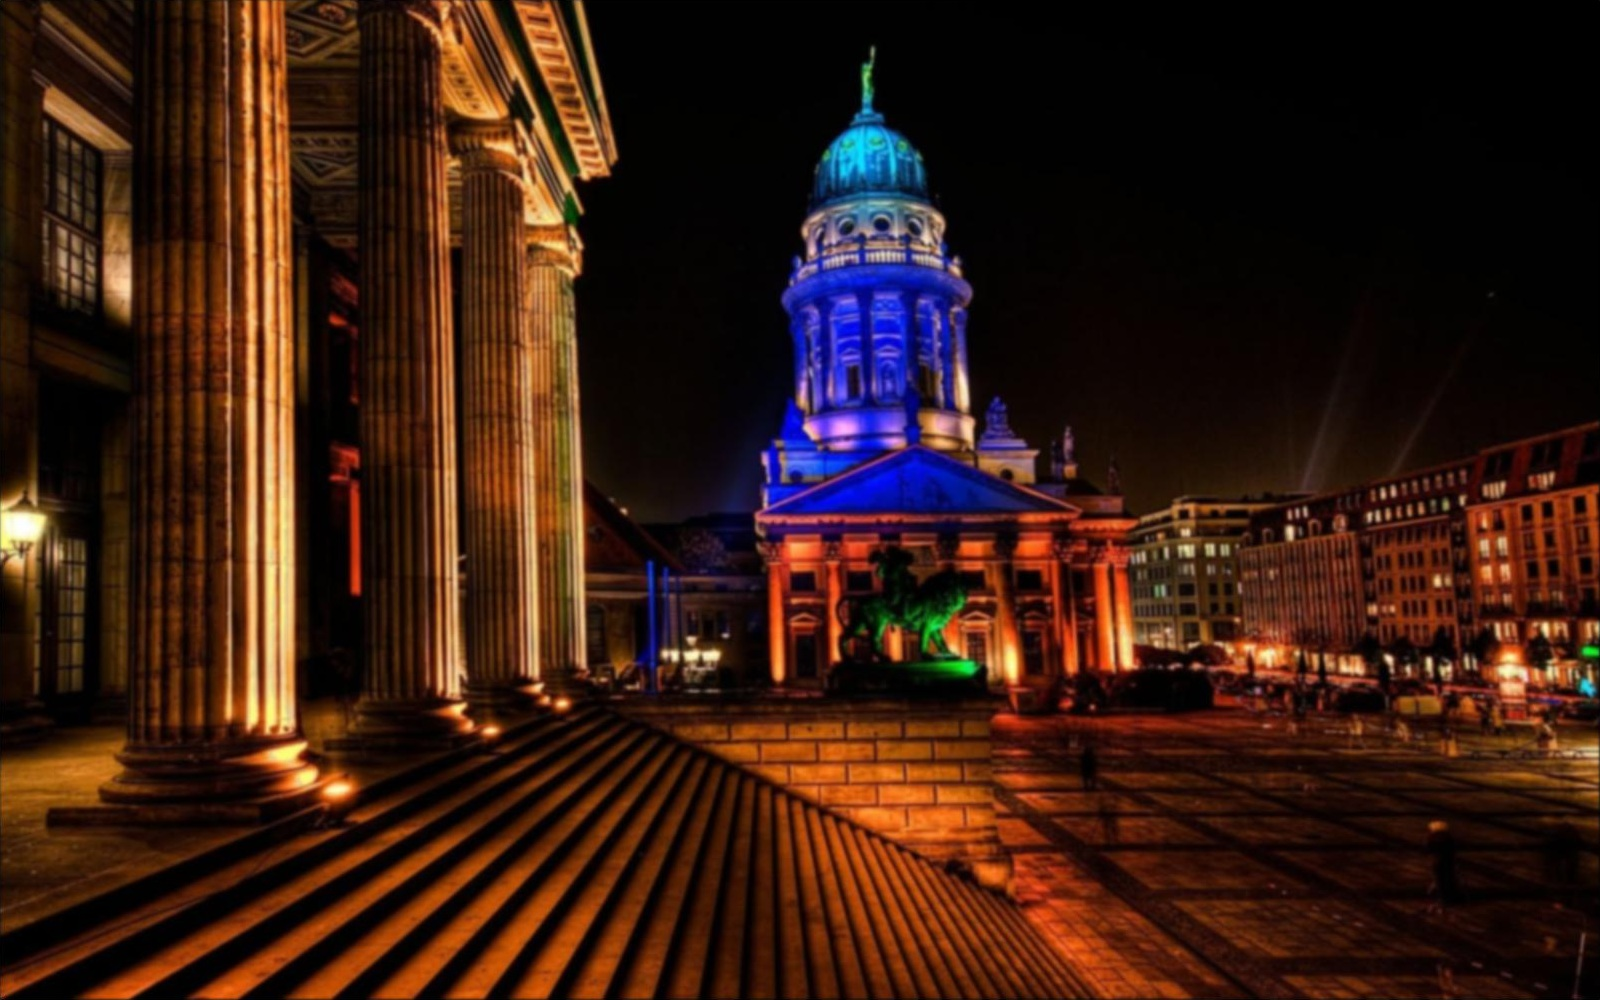
\includegraphics[width=35mm,height=35mm]{cityBlurry.jpg}  
		\label{fig:cityBlurry}
	}	
	\subfigure[Blockiness = 0.0231]{
		\centering
		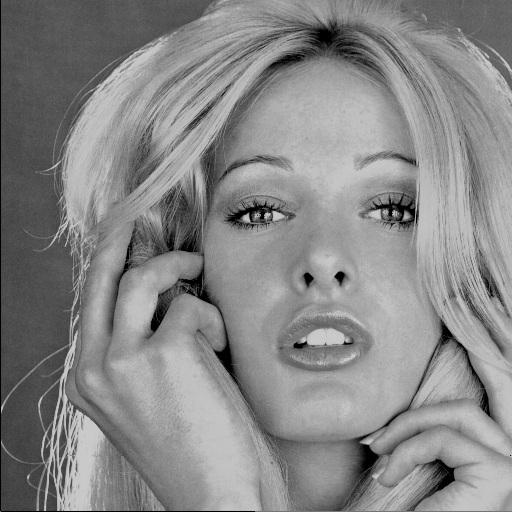
\includegraphics[width=35mm,height=35mm]{tiffanyOriginal.jpg}  
		\label{fig:tiffanyOriginal}	
	}
	\subfigure[Blockiness = 0.6744]{
		\centering
		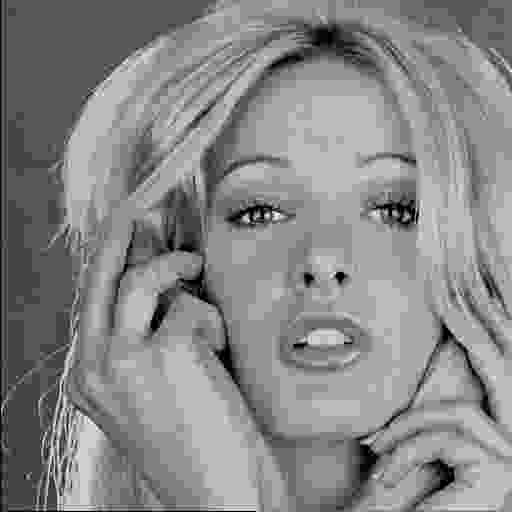
\includegraphics[width=35mm,height=35mm]{tiffanyBlocky.jpg}  
		\label{fig:tiffanyBlocky}
	}
	\caption{Blurriness and Blockiness Results.} \label{fig:BlurrBlockExp}	
\end{figure}

\subsubsection{Blockiness}

Our implementation of the Blockiness algorithm was based on a paper by Wang et al \cite{Wang}.  
The blockiness algorithm is designed as a No-Reference quality measurement algorithm for JPEG compressed images.  
Blockiness is estimated as the average difference across block boundaries.  
$B_{h}$ is the horizontal blockiness and $B_{v}$ is the vertical blockiness.

\begin{equation}
B_{h}=\frac{1}{M([N/8]-1)} \sum_{i=1}^{M} \sum_{j=1}^{[N/8]-1} |d_{h}(i,8j)|
\end{equation}

\begin{equation}
d_{h}(m,n)=x(m,n+1)-x(m,n)
\end{equation}

\begin{equation}
B_{v}=\frac{1}{N([M/8]-1)} \sum_{i=1}^{[M/8]-1} \sum_{j=1}^{N} |d_{v}(8i,j)|
\end{equation}

\begin{equation}
d_{v}(m,n)=x(m+1,n)-x(m,n)
\end{equation}

\noindent The final blockiness model is given in the equation below.  We used a value of 0.01 for $\beta$ and 1.0 for $\gamma$.
We also took into account the activity of the image signal as discussed in the paper \cite{Wang}.
The blockiness extent is demonstrated in Figure (\ref{fig:tiffanyOriginal}) and Figure (\ref{fig:tiffanyBlocky}).

\begin{equation}
S=\beta \left(\frac{B_{h}+B{v}}{2}\right)^\gamma
\end{equation}

















\subsection{Panorama Discovery}

Panorama discovery is defined as finding frames in a video that constitutes a panorama.  
Videos may contain frames that are not panoramic source images.  
We consider a video segment with the following properties to be a valid panorama source.  
A video segment is defined as a series of sequential frames.  There may be multiple video segments within a shot.

\vspace{5 mm}

\noindent\textbf{Property 1}: A video segment should cover a wide field-of-view based on the definition of panorama imagery.

\vspace{5 mm}

\noindent\textbf{Property 2}: A video segment should be �mosaicable�.  
Specifically, the underlying camera motion between frames should observe a certain camera motion model.  
We use a homography to model the motion between frames.  This property should be met after the shot detection algorithm.

\vspace{5 mm}

\noindent\textbf{Property 3}: The frames in a video segment should have high image quality.  
This conservative strategy is adopted so we can ignore methods to improve image visual quality, such as de-blurring and de-blocking.

\vspace{5 mm}

Ideally, we want to discover panoramas that have a very wide field-of-view and are of very high visual quality.  
Unfortunately, there is a tradeoff in practice.  More frames need to be included in order to have a wider field-of-view.  
However, including more source frames can often degrade the visual quality due to motion estimation error.  
We formulate discovering panoramas from a video shot as an optimization problem.  
The optimization problem aims to find a series of video segments that achieve an optimal balance between maximizing 
the visual quality of the resulting panoramas and maximizing the scenes they cover.  We implemented a variation
of the original optimization problem presented in the paper by Liu et al \cite{Feng}.  An overview of the orginal optimization problem is
described below followed by a detailed explaination of our modified optimization problem.  Lastly, our implementation
is discussed in greater detail.

\subsubsection{Original Optimization Problem}

The original optimization problem presented in the paper by Liu et al \cite{Feng} is shown in (\ref{eq:OrgOptEqu}).
Directly solving the constrained nonlinear programming problem is difficult.  
In fact the authors of the paper approximated the optimal solution.  Details of 
their approximation is discussed in paper.


% OPTIMIZATION PROBLEM
% FIRST LINE
\begin{equation} 
\hat{S}=arg \displaystyle\min_{S}
\{ \sum_{S_{i}\epsilon S} E_{v}(S_{i}) + \sum_{S_{i},S_{j}\epsilon S} E_{a}(S_{i},S_{j}) \} \label{eq:OrgOptEqu}
\end{equation}
% SECOND LINE
\begin{equation*}
where \; S=\{ S_{i} \mid S_{i} \subseteq V \}, \;
\forall S_{i},S_{j} \epsilon S, \;
S_{i} \cap S_{j} = {\o}
\end{equation*}
% THIRD LINE
\begin{equation*}
s.t. \left\{ \begin{array}{l}
E_{v}(S_{i}) < \delta , \forall S_{i} \epsilon V \\
\varepsilon(S_{i}) > \beta A , \forall S_{i} \epsilon V
\end{array} \right.
\nonumber
\end{equation*}

\vspace{5 mm}

$S$ denotes a set that contains non-overlapping segments $S_{i}$ of the video clip $V$.
$E_{v}(S_{i})$ is the visual quality cost of stitching a panorama from $S_{i}$, and
$E_{a}(S_{i},S_{j})$ is the cost of splitting a panorama from $S_{i} \cup S_{j}$ into smaller
ones from $S_{i}$ and $S_{j}$ respectively.  $\varepsilon(S_{i})$ denotes the extent of the scene
in $S_{i}$, which is required to be bigger than $\beta$ times the original video frame
size $A$.  To gaurantee the visual quality of the panorama, the visual quality distortion
$E_{v}(S_{i})$ is required to be less than a threshold $\delta$.

\subsubsection{Modified Optimization Problem}

We relaxed the optimization problem as shown in equation (\ref{eq:OrgOptEqu}) to the two step problem shown in equations (\ref{eq:OurOptEqu1}) and (\ref{eq:OurOptEqu2}).
This difference provides our final algorithm with a major benefit.  The benefit is that $E_{a}(S_{i},S_{j})$, the cost of splitting a panorama, 
is no longer considered in Step 1, which reduces the computational difficulty.  Instead Step 2 aims to merge segments that greatly overlap.  
In our modified optimization problem we consider overlapping segments $S_{i}$ of the video clip $V$ as part of the set $S$.  The parameter $\alpha$
is used to tune the extent of overlap required for segments to be merged.  This is useful because to some extent identifying panoramas is
subjective to the user.  This will be discussed in greater detail in Section (\ref{sec:PanDiscExpSec}).


\vspace{5 mm}

\noindent\textbf{Step 1:}
% FIRST LINE
\begin{equation}
\hat{S}=arg \displaystyle\min_{S} \{ \sum_{S_{i}\epsilon S} E_{v}(S_{i}) \} \label{eq:OurOptEqu1}
\end{equation}
% SECOND LINE
\begin{equation*}
where \; S=\{ S_{i} \mid S_{i} \subseteq V \} 
\end{equation*}
% FOURTH LINE
\begin{equation*}
s.t. \left\{ \begin{array}{l}
E_{v}(S_{i}) < \delta , \; \forall \; S_{i} \epsilon V \\
\varepsilon(S_{i}) > \beta A , \; \forall \; S_{i} \epsilon V
\end{array} \right.
\end{equation*}

\vspace{5 mm}

\noindent\textbf{Step 2:}
% FIRST LINE
\begin{equation}
P = 2^{S} \label{eq:OurOptEqu2}
\end{equation}
% SECOND LINE
\begin{equation*}
s.t. \{ \varepsilon(P_{i} \cap P_{j}) < min(\alpha \varepsilon(P_{i}),\alpha \varepsilon(P_{j})), \; \forall \; P_{i},P_{j} \epsilon V
\end{equation*}

\vspace{5 mm}

$S$ denotes a set that may contain overlapping segments $S_{i}$ of the video clip $V$.
$E_{v}(S_{i})$ is the visual quality cost of stitching a panorama from $S_{i}$.
$\varepsilon(S_{i})$ denotes the extent of the scene or total area in $S_{i}$, which is required to be bigger than $\beta$ times the original video frame
size $A$.  To gaurantee the visual quality of the panorama, the visual quality distortion
$E_{v}(S_{i})$ is required to be less than a threshold $\delta$.
$P$ is the power set of $S$ that meets the constraint of equation (\ref{eq:OurOptEqu2}).  The constraint is for any two subsets $P_{i},P_{j}$
of $P$, the area of their intersection must be less than $\alpha \varepsilon(P_{i})$ and $\alpha \varepsilon(P_{j})$.
P is the final set of panoramas, which may contain overlapping segments.

As mentioned, $E_{v}(S_{i})$ is the visual quality cost of stitching a panorama from $S_{i}$.  This is measured from two
aspects: the incorrectness of the motion model denoted as $E_{vm}(S_{i})$, and the source image visual quality distortion
denoted as $E_{vv}(S_{i})$.

\begin{equation}
E_{v}(S_{i}) = \alpha_{m} E_{vm}(S_{i}) + \alpha_{v} E_{vv}(S_{i}) \label{eq:Ev}
\end{equation}

\noindent where $\alpha_{m}$ and $\alpha_{v}$ are weights, with default values 1.0 and 1.0.

The motion model usually cannot be perfectly accurate when describing the correspondence between two frames.  Since we use
a homography for our motion model, homography error is used to measure the incorrectness of the motion model.  $E_{vm}(S_{i})$ is 
the sum of the homography errors between adjacent frames in $S_{i}$ as shown in equation (\ref{eq:Evm}).

\begin{equation}
E_{vm}(S_{i}) = \sum_{I_{k},I_{k+1} \epsilon S_{i}} H_{error}(I_{k},I_{k+1}) \label{eq:Evm}
\end{equation}

\noindent where $I_{k}$ is a frame and $H_{error}$ is the homography error between two adjacent frames.  Homography error 
calculation is discussed in Section (\ref{sec:HomoSec}).

Source frames often suffer from compression distortion.  We measure the input visual quality distortion using the blockiness and
blurriness discussed in Section (\ref{sec:BlurBlockSec}).  $E_{vv}(S_{i})$ is the sum of weighted blurriness extent and blockiness extent 
of each frame in $S_{i}$ as shown in equation (\ref{eq:Evv}).

\begin{equation}
E_{vv}(S_{i}) = \sum_{I_{k} \epsilon S_{i}} \gamma q_{bk}(I_{k}) + (1 - \gamma) q_{bk}(I_{k}) \label{eq:Evv}
\end{equation}

\noindent where $q_{bk}(I_{k})$ and $q_{br}(I_{k})$ measure the blockiness and blurriness of frame $I_{k}$, and 
$\gamma$ is a parameter with the default value 0.45.

\subsubsection{Implementation}

Our implementation is discussed in greater detail due to the complexity of the optimization problem.  The first step in our implementation is to
find the set $S$.  $S_{i}$ candidates are determined by selecting a reference frame as shown in Figure (\ref{fig:referenceFrame})
and then appending adjacent frames until the threshold $\delta$ is met.  All possible reference frames are considered to 
ensure a complete solution.  The set $S$ is determined from the set of $S_{i}$ candidates by verifying the scene extent is sufficient.
The second step is to merge video segements $S_{i}$ that greatly overlap.  The parameter $\alpha$ is used to tune the extent of overlap.
The set of segments $P$ are the discovered panoramas.

\begin{enumerate}
\item[I.] Determine the set $S$
\begin{enumerate}
\item[1.] Select a Reference Frame $I_{k}$ and place it in set $S_{i}$.
\item[2.] Determine the left most frame $I_{l}$ and right most frame $I_{r}$ in set $S_{i}$.
\item[3.] Find the minimum of $E_{v}(I_{l})$ and $E_{v}(I_{r})$.
\item[4.] Add $I_{l}$ or $I_{r}$ to the set $S_{i}$ depending on the results of the previous step.
\item[5.] Repeat steps 2 - 4 until the error threshold $\delta$ is met.
\item[6.] If $\varepsilon (S_{i}) > \beta A$ then add $S_{i}$ to $S$.  
\item[7.] Repeat steps 1 - 6 for all possible Reference Frames.
\end{enumerate}
\item[II.] Determine the set $P$
\begin{enumerate}
\item[1.] Find the power set of $S$ so that Equation (\ref{eq:OurOptEqu2}) is satisfied.
\end{enumerate}
\end{enumerate}

\begin{figure}[H] 
  \centering
  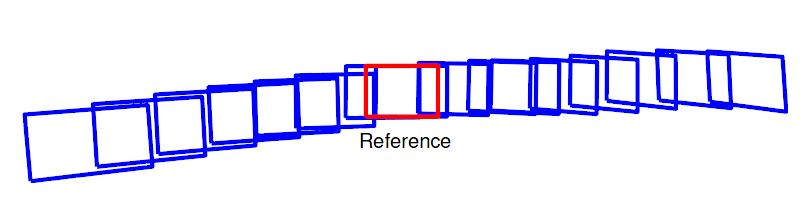
\includegraphics[scale=0.4]{referenceFrame.jpg}  
  \caption{All the frames in the video segment are aligned to the reference frame (in red).  
  The union of all these aligned quadrilaterals is the area covered by the video segment. \cite{Feng}} \label{fig:referenceFrame}
\end{figure}










\subsection{Image Stitching} \label{sec:ImageStitch}
Image stitching consisted of two main parts; aligning individual images together based off of the homographies 
and then blending the aligned images together into the final panorama. 

\subsubsection{Alignment}
Image alignment depends solely on the homography between two individual frames. In our implementation we 
calculate the homography between two consecutive frames and extract the associated translations; this allows
us to align the images in preparation for blending later on. From the homography calculation, we disregard
any knowledge of skew and rotation and thus maintain the rectangular proportion of each frame. This allows 
alignment to be simplified in addition to easier blending calculations explained in the next section.

\subsubsection{Blending}
Image blending is an important part of the stitching process. The method used in blending directly relates to
the quality of the final panorama produced. The blending process we utilized consisted of three steps, taking
a distance-weighted average for each pixel value, median-bilateral filtering, and incorporating the visual 
quality measurement. The overlapping area between frames consist of multiple pixels that need to blended 
together. The overall equation that is used is as follows:
\begin{equation}
I^P(X)=\displaystyle\sum_{k} w_k(x)\tilde{I}_k(x)/\displaystyle\sum_{k} w_k(x)
\end{equation}

Where $I_P(X)$ is the pixel value at index $x$ for panorama number $P$, $w_k(x)$ is the weighting for the 
pixel at index $x$ in frame number $k$, and $\tilde{I}_k(x)$ is the intensity of the pixel at index $x$ in 
it's corresponding frame $k$. The weighting for each pixel is the product of three calculations:
\begin{equation}
w_k(x) = w_{k1}(x)w_{k2}(x)w_{k3}(x)
\end{equation}

The final weighting for each pixel is the product of three calculations, $w_{k1}(x)$ is the shortest horizontal 
distance of the pixel $x$ from the nearest vertical edge; this is done to give more weight to those pixels to 
the center of the image than those at the edge. This calculation is represented by the following equation:
\begin{equation}
w_{k1}(x) =  \| \text{arg} \displaystyle\min_{y}\{\|y\|\; \tilde{I}_k (x+y) \text{ is invalid} \}\|
\end{equation}

Following which $w_{k2}(x)$ is the weighting as a result of a median-bilateral filter which takes into account
the average (median) value of all the pixels that overlap, from different frames, in the final panorama; this
is calculated using the equation shown below:
\begin{equation}
w_{k2}(x) = exp (-(\tilde{I}_k(x)-med(x))^2/\sigma^2)
\end{equation}

Lastly, the third term of the weight calculation, $w_{k3}(x)$, takes into account the individual quality of 
each frame that the pixel belongs to. The pixels that come frame a frame that is of a higher quality contribute
a higher weight to the final result; this is shown in the equation below:
\begin{equation}
w_{k3}(x) = exp (-(\gamma q_{bk}(k) + (1 - \gamma)q_{br}(k)))
\end{equation}

This blending method is applied to each color (RGB) in turn and the resulting image is the blended panorama.





\section{Experiments}

The experimental results of our panorama discovery algorithm is shown in Section (\ref{sec:PanDiscExpSec}), and blending algorithm is
shown in Section (\ref{sec:BlendExpSec}).

\subsection{Panorama Discovery} \label{sec:PanDiscExpSec}

Panorama discovery is defined as finding frames in a video that constitutes a panorama.
The solution may be subjective.  An example is shown in Figure (\ref{fig:archResults}).
An argument can be made that there should be only one panorama.  However, the quality of the 
panorama may suffer due to the motion model error.  The parameters can be tuned, specifically
$\delta$ and $\beta$, to get different results.

The implemented panorama discovery algorithm is robust enough to account for the 
video zoom.  An example is shown in Figure (\ref{fig:vancouverResults}).

\end{multicols}

\begin{figure} [t]
	\centering
	\subfigure[Panorama 1.]{
		\centering
		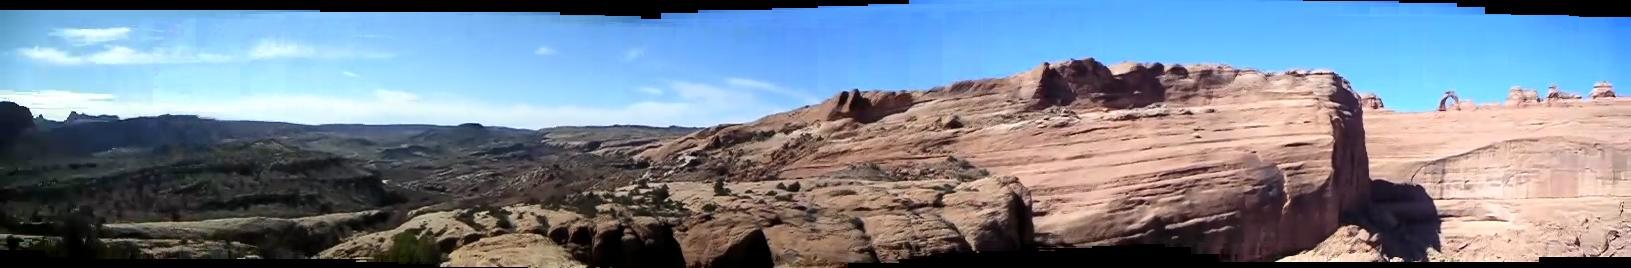
\includegraphics[width=170mm,height=30mm]{archPan1.jpg}  
		\label{fig:archPan1}
	}	
	\subfigure[Panorama 2.]{
		\centering
		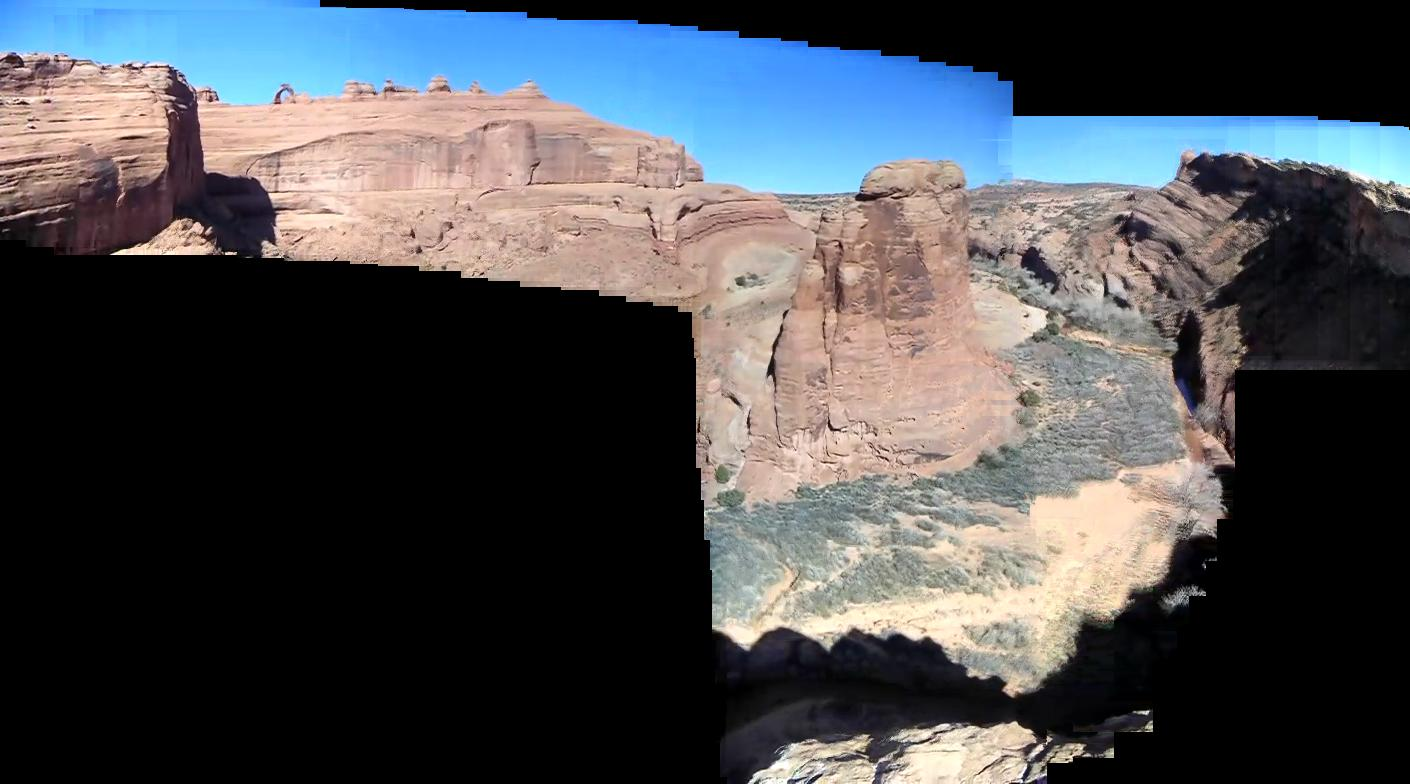
\includegraphics[width=170mm,height=80mm]{archPan2.jpg}  
		\label{fig:archPan2}	
	}
	\caption{Discovered Panoramas from a Web Video \cite{Arches}.} \label{fig:archResults}	
\end{figure}

\begin{figure} [H]
	\centering
	\subfigure[Panorama 1.]{
		\centering
		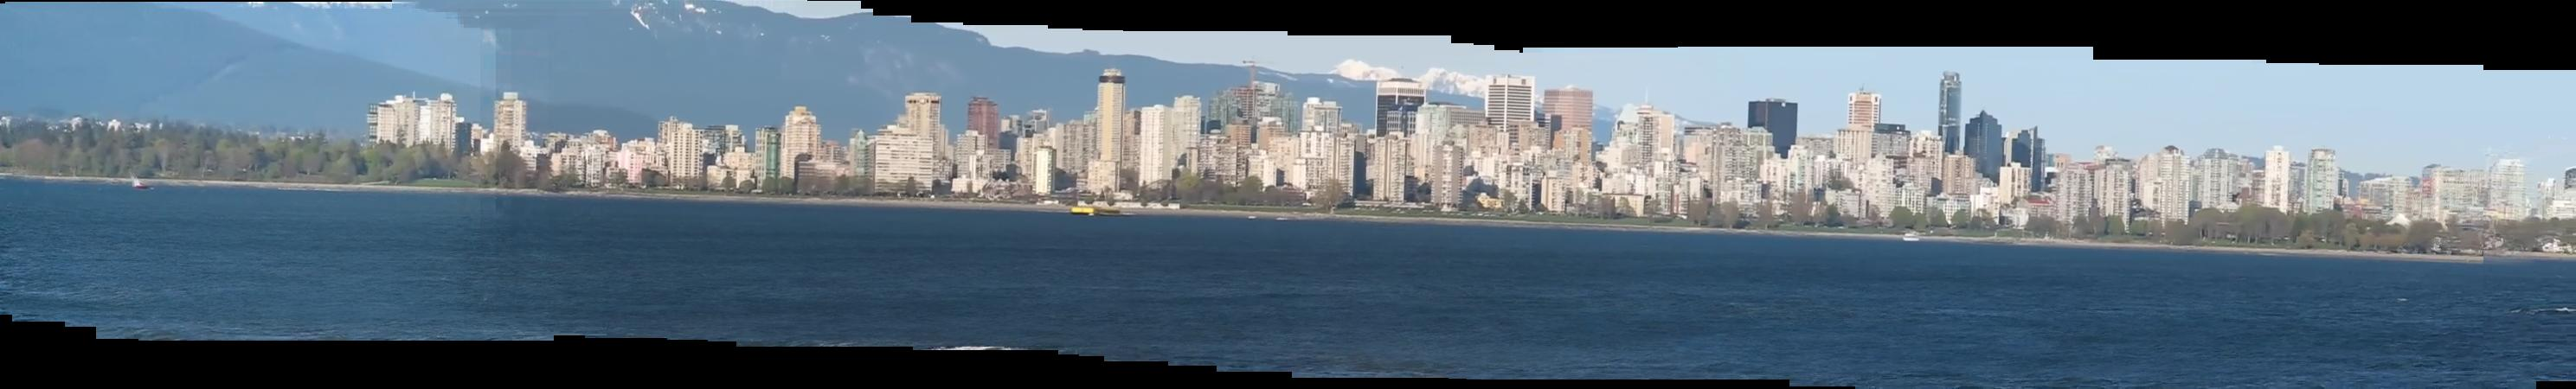
\includegraphics[width=170mm,height=30mm]{vancouverPan1.jpg}  
		\label{fig:vancouverPan1}
	}	
	\subfigure[Panorama 2.]{
		\centering
		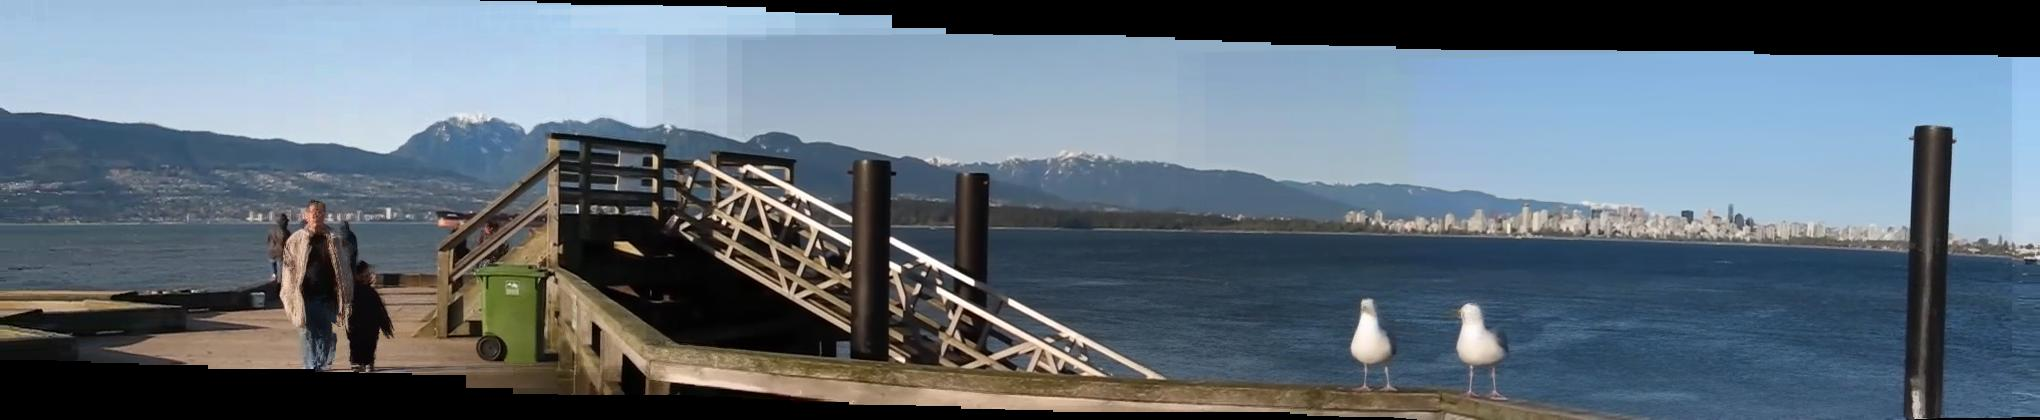
\includegraphics[width=170mm,height=30mm]{vancouverPan2.jpg}  
		\label{fig:vancouverPan2}	
	}
	\caption{Discovered Panoramas from a Web Video \cite{Vancouver}.} \label{fig:vancouverResults}	
\end{figure}

\begin{multicols}{2}

\end{multicols}

% Figures for Blending
\begin{figure} [H]
	\centering
	\subfigure[Without Median-Bilateral Filter.]{
		\centering
		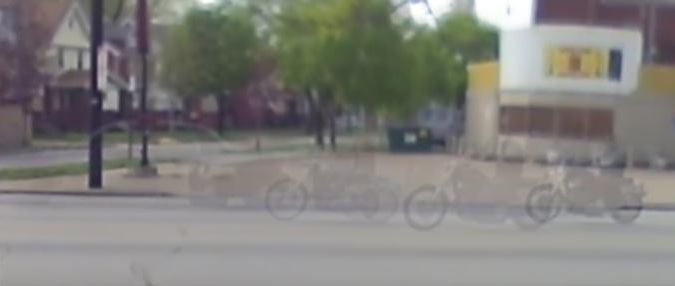
\includegraphics[width=70mm,height=40mm]{withoutFilter.jpg}  
		\label{fig:withoutFilter}
	}	
	\subfigure[With Median-Bilateral Filter.]{
		\centering
		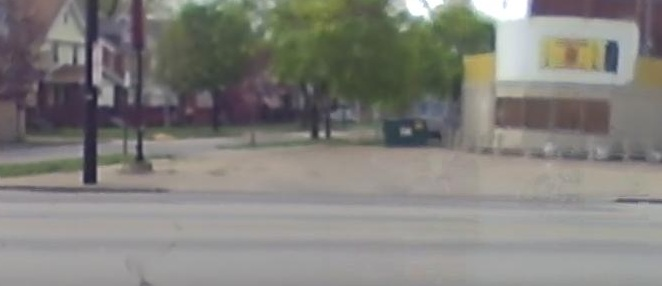
\includegraphics[width=70mm,height=40mm]{withFilter.jpg}  
		\label{fig:withFilter}	
	}
	\caption{Effects of the median-bilateral filter on the final stitched image.} \label{fig:BlendFilterExp}	
\end{figure}

\begin{multicols}{2}

\subsection{Blending} \label{sec:BlendExpSec}

We implemented a three stage blending algorithm as discussed in Section (\ref{sec:ImageStitch}).  
The first stage is a feathering algorithm, common for stitching panoramas.
Feathering algorithms tend to leave ghosting artifacts shown in Figure (\ref{fig:withoutFilter}).
Ghosting artifacts are a result of moving objects between frames.  This is a major problem since we use videos as our panorama sources.
Videos tend to have moving objects.  Our solution was to implement a median-bilateral filter in the second stage.
The median-bilateral filter mitigates ghosting artifacts as shown in Figure (\ref{fig:withFilter}).






\section{Conclusion}

In this project, we have analyzed web videos as a panorama source. We implemented an automatic method to discover panorama sources from casual videos. 
The panorama sources should satisfy three properties, namely wide field-of-view, mosaicabilty and high image quality. Based on these properties, we formulate discovery of panoramas as an 
optimization problem that tries to achive an optimum balance between maximizing the visual quality of the resulting panoramas and maximizing the scenes that the panoramas cover. We have relaxed the original 
optimization problem to reduce the computational complexity. After finding these panorama sources, we stitch it to create scene panorama. 
In this project, we analyzed the feasibility of using web videos to create good quality panoramas. We have been successful in finding panoramas for a large number of casual videos.  We also found that the quality of panorama was dependent on the video quality
and the movement of the camera. Our method could be improved to include videos with skew, zoom and large camera rotations. Nevertheless, our method has been effecient to create interesting panoramas from web videos.

\begin{thebibliography}{99}

  
\bibitem{Feng} Feng Liu, Yu-hen Hu and Michael Gleicher. Discovering panoramas in web videos. 
ACM Multimedia 2008, Vancouver, Canada, October 2008. pp. 329-338.  

\bibitem{Tong} H. Tong, M. Li, H. Zhang, and C. Zhang. Blur
detection for digital images using wavelet transform.
In IEEE ICME, 2004.

\bibitem{Wang} Z. Wang, H. Sheikh, and A. Bovik. No-reference
perceptual quality assessment of jpeg compressed
images. In IEEE ICIP, pages Vol I: 477-480, 2002.

\bibitem{Lien} Lienhart, Rainer. Comparison of automatic shot boundary detection algorithms.

\bibitem{Lowe} David Lowe. SIFT Keypoint Detector.
http://www.cs.ubc.ca/~lowe/keypoints/.

\bibitem{Arches} Delicate Arch.  Retrieved December 15, 2012,
http://www.youtube.com/watch?v$=$ZMbr8uRk3nM.

\bibitem{Vancouver} Jericho Beach in Vancouver British Columbia.  Retrieved December 15, 2012,
http://www.youtube.com/watch?v$=$BrUgzmgDVw8.

\bibitem{YouTube} YouTube. http://www.youtube.com/

\bibitem{Picasa} Picasa. http://picasa.google.com/

\bibitem{Vimeo} Vimeo. http://vimeo.com/




\end{thebibliography}


\end{multicols}


\end{document}
